\documentclass[12pt]{article}
\usepackage[utf8]{inputenc}
\usepackage{ulem}
\usepackage[english,russian]{babel}
\usepackage{amssymb}
\usepackage{graphicx}
\usepackage{setspace}
\usepackage{geometry}
\usepackage[english]{blindtext}
\usepackage[matrix,arrow,curve,frame,poly,arc]{xy}
\usepackage{fancyhdr}
\usepackage{subcaption}
\usepackage[export]{adjustbox}
\usepackage{wrapfig}
\usepackage{amsmath}
\usepackage{subfig}
\graphicspath{ {image} }
\usepackage{hyperref}
\hypersetup{pdfstartview=FitH,  linkcolor=linkcolor,urlcolor=urlcolor, colorlinks=true}

\begin{document}

    \begin{titlepage}
        \thispagestyle{empty}
        \begin{center}
            \noindent\begin{minipage}{0.14\textwidth}
                         
\includegraphics[width=\linewidth]{image/madi_logo}
            \end{minipage}%
            \begin{minipage}{0.86\textwidth}
                \center{\small{\vspace{\baselineskip}}}
                \center{{МИНИСТЕРСТВО НАУКИ И ВЫСШЕГО ОБРАЗОВАНИЯ РОССИЙСКОЙ ФЕДЕРАЦИИ \\ федеральное бюджетное образовательное государственное учреждение высшего образования}
                    \center{{\hspace{1 cm}}}}
            \end{minipage}
            \small{\textbf{<<МОСКОВСКИЙ АВТОМОБИЛЬНО-ДОРОЖНЫЙ ГОСУДАРСТВЕННЫЙ ТЕХНИЧЕСКИЙ УНИВЕРСИТЕТ (МАДИ)>>}}\\
            \vspace{0.2 cm}
            \scriptsize{{\textbf{КАФЕДРА <<ВЫСШАЯ МАТЕМАТИКА>> }}}
            \vspace{\baselineskip}

            \small{\textbf{КУРСОВАЯ РАБОТА}}\\
            \vspace{0.2 cm}

            по дисциплине <<<Базы данных>>
            на тему\\
            <<Приложения на Android с подключенной базой данных. >>
        \end{center}

        \hfill \begin{minipage}{0.5\linewidth}
                   \textbf{Выполнил:}\\
                   Учебная группа 2бПМ\\
                   Осада.В.В\\
                   Акилин.Я.А\\
                   \textbf{Руководитель курсового проекта:
                   }\\
                   Старший преподаватель\\
                   Кутейников.И.А\\
                   Подпись \underline{\hspace{1cm}}\\
        \end{minipage}
        \vspace{1 cm}
        \begin{minipage}{0.45\linewidth}
            Курсовой проект защищен\\ с оценкой <<\underline{\hspace{1cm}}>>\\
            <<\underline{\hspace{0.7cm}}>> \underline{\hspace{2cm}} 2023 г.
        \end{minipage}
        \begin{minipage}{0.55\linewidth}
        \end{minipage}
        \vspace{5 cm}
        \center{Москва 2023}
    \end{titlepage}

    \tableofcontents
    \newpage

    \section{Введение}
    В современном мире мобильные приложения являются неотъемлемой частью нашей повседневной жизни. Они предоставляют удобный способ взаимодействия с информацией и облегчают выполнение различных задач. Одной из самых популярных платформ для разработки мобильных приложений является Android, предлагающий множество возможностей для создания функциональных и эффективных приложений.

    В данной курсовой работе представляется Android приложение, разработанное для кафедры физкультуры, которое позволяет вносить и хранить данные о матчах по волейболу вузовской команды. Приложение основано на подключенной базе данных, что обеспечивает надежное хранение и управление данными, а также позволяет осуществлять различные операции с информацией о матчах.

    \section{Цель проекта}
    Целью разработки данного приложения является автоматизация процесса сбора и анализа статистических данных о матчах волейбольной команды. Приложение предоставляет удобный интерфейс для ввода информации о матчах, включая дату, противника, счет, статистику игроков и другие параметры. Собранные данные могут быть использованы для анализа результатов команды, оценки эффективности игроков, определения трендов и принятия решений по улучшению игры.

    В дальнейшей части работы будет рассмотрена архитектура приложения, подходы к подключению базы данных, процесс разработки интерфейса пользователя, функциональные возможности приложения, а также примеры кода для более подробного понимания реализации. Также будет проведен анализ результатов использования приложения и обсуждены возможности для его дальнейшего улучшения.

    \section{Основная часть}
    \subsection{Реализация главного меню и переход на статистику игрока}

    В рамках нашего проекта мы успешно реализовали главное меню, которое является входной точкой для пользователей приложения. Главное меню разработано с использованием XML-разметки, что позволяет нам легко определить и настроить внешний вид интерфейса.

    На главном меню содержится 6 кнопок, каждая из которых соответствует выбору определенного игрока. При нажатии на любую из этих кнопок происходит переход на экран со статистикой данного игрока. Такой подход позволяет пользователям быстро и удобно получать информацию о производительности каждого игрока.

    Ниже приведен пример кода XML-разметки для главного меню:

    \begin{verbatim}
    <?xml version="1.0" encoding="utf-8"?>
<androidx.constraintlayout.widget.ConstraintLayout xmlns:android="http://schemas.android.com/apk/res/android"
    xmlns:app="http://schemas.android.com/apk/res-auto"
    xmlns:tools="http://schemas.android.com/tools"
    android:layout_width="match_parent"
    android:layout_height="match_parent"
    tools:context=".MainActivity"
    android:background="#563C31">

    <LinearLayout
        android:layout_width="match_parent"
        android:layout_height="match_parent"
        android:orientation="horizontal"
        android:gravity="top"
        tools:context=".MainActivity">

        <!-- Кнопка 1 -->
        <Button
            android:id="@+id/button1"
            android:layout_width="wrap_content"
            android:layout_height="wrap_content"
            android:text="0"
            android:layout_weight="1"
            android:backgroundTint="#D9D9D9"
            android:textColor="#000000"/>

        <!-- Кнопка 2 -->
        <Button
            android:id="@+id/button2"
            android:layout_width="wrap_content"
            android:layout_height="wrap_content"
            android:text="0"
            android:layout_weight="1"
            android:backgroundTint="#D9D9D9"
            android:textColor="#000000"/>

    </LinearLayout>

    <LinearLayout
        android:layout_width="match_parent"
        android:layout_height="match_parent"
        android:orientation="vertical"
        android:gravity="top"
        android:layout_marginTop="100dp"
        tools:context=".MainActivity">

        <Button
        android:id="@+id/button4"
        android:layout_width="wrap_content"
        android:layout_height="wrap_content"
        android:text="Player 1"
        android:layout_weight="1"
        android:backgroundTint="#D9D9D9"
        android:textColor="#000000"/>

        <Button
            android:id="@+id/button5"
            android:layout_width="wrap_content"
            android:layout_height="wrap_content"
            android:text="Player 2"
            android:layout_weight="1"
            android:backgroundTint="#D9D9D9"
            android:textColor="#000000">
            </Button>

        <Button
            android:id="@+id/button6"
            android:layout_width="wrap_content"
            android:layout_height="wrap_content"
            android:text="Player 3"
            android:layout_weight="1"
            android:backgroundTint="#D9D9D9"
            android:textColor="#000000">
            </Button>

        <Button
            android:id="@+id/button7"
            android:layout_width="wrap_content"
            android:layout_height="wrap_content"
            android:text="Player 4"
            android:layout_weight="1"
            android:backgroundTint="#D9D9D9"
            android:textColor="#000000">
            </Button>

        <Button
            android:id="@+id/button8"
            android:layout_width="wrap_content"
            android:layout_height="wrap_content"
            android:text="Player 5"
            android:layout_weight="1"
            android:backgroundTint="#D9D9D9"
            android:textColor="#000000">
            </Button>

        <Button
            android:id="@+id/button9"
            android:layout_width="wrap_content"
            android:layout_height="wrap_content"
            android:text="Player 6"
            android:layout_weight="1"
            android:backgroundTint="#D9D9D9"
            android:textColor="#000000">
        </Button>
    </LinearLayout>

    <LinearLayout
        android:layout_width="match_parent"
        android:layout_height="match_parent"
        android:orientation="vertical"
        android:gravity="end"
        android:layout_marginTop="90dp">
        <Button
            android:layout_marginTop="10dp"
            android:id="@+id/button10"
            android:layout_width="wrap_content"
            android:layout_height="wrap_content"
            android:text="ACE"
            android:layout_weight="1"
            android:backgroundTint="#A8C4DC"
            android:textColor="#000000">
        </Button>

        <Button
            android:layout_marginTop="10dp"
            android:id="@+id/button11"
            android:layout_width="wrap_content"
            android:layout_height="wrap_content"
            android:text="SPIKE"
            android:layout_weight="1"
            android:backgroundTint="#A8C4DC"
            android:textColor="#000000">
        </Button>

        <Button
            android:layout_marginTop="10dp"
            android:id="@+id/button12"
            android:layout_width="wrap_content"
            android:layout_height="wrap_content"
            android:text="TIP"
            android:layout_weight="1"
            android:backgroundTint="#A8C4DC"
            android:textColor="#000000">
        </Button>

        <Button
            android:layout_marginTop="10dp"
            android:id="@+id/button13"
            android:layout_width="wrap_content"
            android:layout_height="wrap_content"
            android:text="DUMP"
            android:layout_weight="1"
            android:backgroundTint="#A8C4DC"
            android:textColor="#000000">
        </Button>

        <Button
            android:layout_marginTop="10dp"
            android:id="@+id/button14"
            android:layout_width="wrap_content"
            android:layout_height="wrap_content"
            android:text="DBH"
            android:layout_weight="1"
            android:backgroundTint="#A8C4DC"
            android:textColor="#000000">
        </Button>

        <Button
            android:layout_marginTop="10dp"
            android:id="@+id/button15"
            android:layout_width="wrap_content"
            android:layout_height="wrap_content"
            android:text="BLOCK"
            android:layout_weight="1"
            android:backgroundTint="#A8C4DC"
            android:textColor="#000000">
        </Button>

    </LinearLayout>



</androidx.constraintlayout.widget.ConstraintLayout>

    \end{verbatim}

    \begin{figure}[ht]
        \centering
        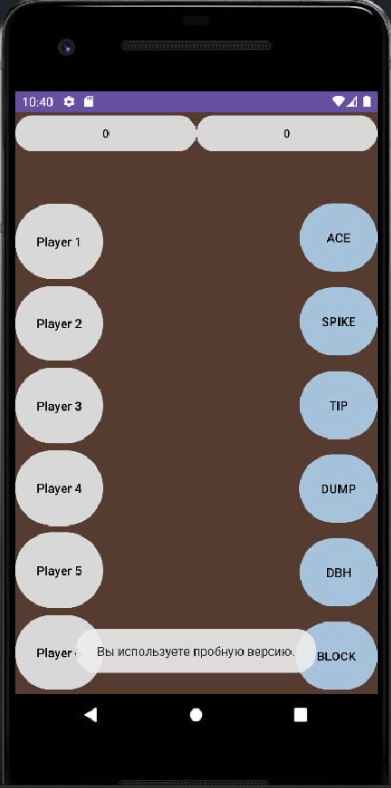
\includegraphics[width=0.3\textwidth]{image/main_menu.png}
        \caption{Скриншот главного меню}
    \end{figure}

    Данный код представляет макет (layout) для разметки пользовательского интерфейса в Android-приложении.
    Внутри <androidx.constraintlayout.widget.ConstraintLayout> определены различные элементы интерфейса, такие как кнопки (Button) и контейнеры (LinearLayout).

    Основной контейнер <LinearLayout> содержит две кнопки (Button), которые располагаются горизонтально.
    Оба Button имеют идентификаторы button1 и button2, текст \("0"\), заданную ширину и высоту, вес равный 1 и цвет фона и текста.

    Последующие <LinearLayout> определяют кнопки для игроков (Player 1, Player 2, и так далее).
    Каждая кнопка имеет уникальный идентификатор, текст, ширину, высоту, вес, цвет фона и текста.

    Контейнер <LinearLayout> с атрибутом gravity="end" располагает кнопки ACE, SPIKE, TIP, DUMP, DBH и BLOCK вертикально внизу экрана.
    Каждая кнопка имеет уникальный идентификатор, текст, ширину, высоту, вес, цвет фона и текста.

    Общий фон экрана установлен с помощью атрибута android:background, где цвет задан в шестнадцатеричном формате (#563C31).

    Этот код представляет только разметку пользовательского интерфейса, и для добавления логики и обработчиков событий, таких как нажатия на кнопки, требуется дополнительный код в классе активности (MainActivity).

    На главном меню также присутствуют кнопки, отвечающие за увеличение и уменьшение счета.
    Эти кнопки позволяют оперативно корректировать текущий счет во время матча.
    Эта функциональность дает пользователям возможность точно отслеживать изменения счета в режиме реального времени.


    \newpage

    \subsection{Логика работы кнопок}
    Этот код представляет класс MainActivity в Android-приложении, который является основной активностью приложения. Вот некоторые комментарии и объяснения для каждого раздела кода:

    1. Импорты:
    \begin{verbatim}

kotlin
import DatabaseHelper
import android.os.Bundle
import android.os.Handler
import android.widget.Toast
import androidx.appcompat.app.AlertDialog
import androidx.appcompat.app.AppCompatActivity
import com.example.myapplication.databinding.ActivityMainBinding
    \end{verbatim}

    Здесь импортируются необходимые классы и пакеты для работы приложения, включая DatabaseHelper (вероятно, пользовательский класс для работы с базой данных), классы для работы с пользовательским интерфейсом (AlertDialog, AppCompatActivity, ActivityMainBinding) и другие.

    2. Определение класса MainActivity:
    \begin{verbatim}

kotlin
class MainActivity : AppCompatActivity() {
    // Переменные для подсчета нажатий на кнопки
    private var countb1 = 0
    private var countb2 = 0

    // Переменные для работы с пользовательским интерфейсом и базой данных
    private lateinit var binding: ActivityMainBinding
    private lateinit var databaseHelper: DatabaseHelper
    private val delayMillis = 10000 // 10 секунд

    // Метод onCreate, вызывается при создании активности
    override fun onCreate(s: Bundle?) {
        super.onCreate(s)
        binding = ActivityMainBinding.inflate(layoutInflater)
        setContentView(binding.root)

        // Создание и отображение диалогового окна AlertDialog
        val alertDialog = AlertDialog.Builder(this)
            .setTitle("Важно")
            .setMessage("Если Вы видите это сообщение, то, вероятно, используете не активированную версию приложения. Перейдите в настройки и введите ключ. tutorchan3@gmail.com.")
            .setPositiveButton("OK") { dialog, _ ->
                dialog.dismiss()
            }
            .create()

        alertDialog.show()

        // Поставщик задержки для показа Toast сообщения
        Handler().postDelayed({
            Toast.makeText(this, "Вы используете пробную версию.", Toast.LENGTH_SHORT).show()
        }, delayMillis.toLong())

        // Обработчики нажатий и долгого нажатия для кнопок button1 и button2
        binding.button1.setOnClickListener {
            countb1++
            binding.button1.text = countb1.toString()
        }

        binding.button2.setOnClickListener {
            countb2++
            binding.button2.text = countb2.toString()
        }

        binding.button1.setOnLongClickListener {
            if (countb1 > 0) {
                countb1--
                binding.button1.text = countb1.toString()
            }
            true
        }

        binding.button2.setOnLongClickListener {
            if (countb2 > 0) {
                countb2--
                binding.button2.text = countb2.toString()
            }
            true
        }

        // Инициализация объекта DatabaseHelper для работы с базой данных
        databaseHelper = DatabaseHelper(this)

        // Обработчик нажатия на кнопку button11 для выполнения операции вставки данных в базу данных
        binding.button11.setOnClickListener {
            databaseHelper.insertButtonPress()


 }
    }

    // Метод onDestroy, вызывается при уничтожении активности
    override fun onDestroy() {
        super.onDestroy()
        // Закрытие базы данных
        databaseHelper.close()
    }
}
    \end{verbatim}

    Основной функционал этого класса включает:
    \begin{itemize}

        \item Создание пользовательского интерфейса, заданного в файле разметки activity_main.xml, используя ActivityMainBinding.
        \item  Отображение AlertDialog с важным сообщением для пользователя.
        \item Подсчет и отображение количества нажатий на кнопки button1 и button2.
        \item Обработка долгого нажатия на кнопки button1 и button2, с уменьшением значения счетчика при каждом долгом нажатии.
        \item Инициализация и использование DatabaseHelper для работы с базой данных.
        \item Обработка нажатия на кнопку button11, которая вызывает метод insertButtonPress() из DatabaseHelper для выполнения операции вставки данных в базу данных.
        \item Закрытие базы данных при уничтожении активности в методе onDestroy().
    \end{itemize}

    \subsection{База данных}

    В нашем приложении мы использовали SQLite, встроенную реляционную базу данных для хранения информации о каждом игроке и их статистику волейбольных матчей. SQLite обладает преимуществами такими, как простота интеграции, надежность, поддержка SQL-запросов и отличная производительность на устройствах Android.

    База данных содержит информацию о каждом игроке, включая:

    \begin{itemize}
        \item Имя игрока: строковое значение, указывающее имя игрока.
        \item Возраст игрока: целочисленное значение, отражающее возраст игрока.
        \item Позиция игрока: строковое значение, указывающее позицию игрока на поле (например, атакующий, блокирующий, либеро и т.д.).
        \item Рост игрока: вещественное значение, отражающее рост игрока в метрах.
        \item Вес игрока: вещественное значение, отражающее вес игрока в килограммах.
        \item Показатели волейбольной статистики: для каждого игрока мы сохраняем показатели, такие как количество сделанных подач, успешных и неуспешных атак, успешных блоков, успешных защит и другие параметры, необходимые для анализа и оценки эффективности игрока.
    \end{itemize}

    Для каждого игрока мы создали соответствующую таблицу в базе данных, где каждое поле таблицы соответствует определенному атрибуту игрока. Мы использовали SQL-запросы для создания таблиц, вставки данных, обновления и извлечения информации из базы данных.

    Преимущества использования SQLite базы данных заключаются в том, что она обеспечивает структурированное хранение информации о каждом игроке, позволяет эффективно выполнять запросы и операции с данными, а также обеспечивает надежность и целостность данных.

    Благодаря использованию SQLite базы данных мы можем сохранять и обрабатывать обширную статистику волейбольных матчей для каждого игрока, что позволяет анализировать результаты команды, оценивать производительность игроков и принимать обоснованные решения для улучшения игры волейбольной команды нашей вузовской кафедры физкультуры.


    \begin{verbatim}
import android.content.Context;
import android.database.sqlite.SQLiteDatabase;
import android.database.sqlite.SQLiteOpenHelper;

public class DatabaseHelper extends SQLiteOpenHelper {
    private static final String DATABASE_NAME = "button_presses.db";
    private static final int DATABASE_VERSION = 1;

    public static final String TABLE_NAME = "button_presses";
    public static final String COLUMN_ID = "id";
    public static final String COLUMN_TIMESTAMP = "timestamp";

    public DatabaseHelper(Context context) {
        super(context, DATABASE_NAME, null, DATABASE_VERSION);
    }

    @Override
    public void onCreate(SQLiteDatabase db) {
        String createTableQuery = "CREATE TABLE " + TABLE_NAME + " (" +
                COLUMN_ID + " INTEGER PRIMARY KEY AUTOINCREMENT, " +
                COLUMN_TIMESTAMP + " DATETIME DEFAULT CURRENT_TIMESTAMP)";
        db.execSQL(createTableQuery);
    }

    @Override
    public void onUpgrade(SQLiteDatabase db, int oldVersion, int newVersion) {
        db.execSQL("DROP TABLE IF EXISTS " + TABLE_NAME);
        onCreate(db);
    }

    public void insertButtonPress() {
        SQLiteDatabase db = getWritableDatabase();
        String insertQuery = "INSERT INTO " + TABLE_NAME + " (" + COLUMN_TIMESTAMP +
                ") VALUES (datetime('now', 'localtime'))";
        db.execSQL(insertQuery);
        db.close();
    }
}

    \end{verbatim}

    Этот код представляет класс DatabaseHelper, который является наследником SQLiteOpenHelper и используется для управления базой данных SQLite в Android-приложении. Вот некоторые объяснения для каждого раздела кода:

    \begin{itemize}

        \item Определение класса DatabaseHelper:
        kotlin
        class DatabaseHelper(context: Context) : SQLiteOpenHelper(context, DATABASE_NAME, null, DATABASE_VERSION) {
            // ...
        }
        Класс DatabaseHelper наследуется от SQLiteOpenHelper и используется для работы с базой данных SQLite. Он принимает контекст приложения в качестве параметра конструктора и передает его в конструктор родительского класса SQLiteOpenHelper.

        \item Определение статических констант:
        \begin{verbatim}

kotlin
companion object {
    private const val DATABASE_NAME = "button_presses.db"
    private const val DATABASE_VERSION = 1

    const val TABLE_NAME = "button_presses"
    const val COLUMN_ID = "id"
    const val COLUMN_TIMESTAMP = "timestamp"
}
Внутри companion object определены константы для имени базы данных (DATABASE_NAME), версии базы данных (DATABASE_VERSION), имени таблицы (TABLE_NAME) и имен столбцов (COLUMN_ID и COLUMN_TIMESTAMP).
        \end{verbatim}


        \item Метод onCreate():
        \begin{verbatim}
kotlin
override fun onCreate(db: SQLiteDatabase) {
    val createTableQuery = "CREATE TABLE $TABLE_NAME ($COLUMN_ID INTEGER PRIMARY KEY AUTOINCREMENT, $COLUMN_TIMESTAMP DATETIME DEFAULT CURRENT_TIMESTAMP)"
    db.execSQL(createTableQuery)
}
Метод onCreate() вызывается при создании базы данных. Внутри него выполняется SQL-запрос для создания таблицы button_presses. Таблица имеет два столбца: id с типом INTEGER в качестве первичного ключа и автоинкрементом, и timestamp с типом DATETIME и значением по умолчанию CURRENT_TIMESTAMP.
        \end{verbatim}

        \item Метод onUpgrade():
        \begin{verbatim}
kotlin
override fun onUpgrade(db: SQLiteDatabase, oldVersion: Int, newVersion: Int) {
    db.execSQL("DROP TABLE IF EXISTS $TABLE_NAME")
    onCreate(db)
}
Метод onUpgrade() вызывается, когда происходит обновление версии базы данных. В данном случае, он выполняет SQL-запрос для удаления существующей таблицы button_presses (если она существует) и затем вызывает onCreate() для создания новой версии таблицы.
        \end{verbatim}

        \item Метод insertButtonPress():
        \begin{verbatim}
kotlin
fun insertButtonPress() {
    val db = writableDatabase
    val insertQuery = "INSERT INTO $TABLE_NAME ($COLUMN_TIMESTAMP) VALUES (datetime('now', 'localtime'))"
    db.execSQL(insertQuery)
    db.close()
}
Метод insertButtonPress() используется для вставки записи в таблицу button_presses. Он получает доступ к базе данных в режиме записи (writableDatabase), формирует SQL-запрос для вставки новой записи с текущим временем (`datetime('now', '

localtime')), выполняет этот запрос с помощью `execSQL(), а затем закрывает базу данных с помощью db.close().
        \end{verbatim}

    \end{itemize}

    Для того, чтобы при нажатии на любую из кнопок разметки происходила запись в базу данных, вам нужно внести изменения в класс MainActivity. Вот код, который добавляет эту функциональность:
    \begin{verbatim}

kotlin
import android.os.Bundle
import android.widget.Button
import android.widget.Toast
import androidx.appcompat.app.AppCompatActivity

class MainActivity : AppCompatActivity() {
    private lateinit var databaseHelper: DatabaseHelper

    override fun onCreate(savedInstanceState: Bundle?) {
        super.onCreate(savedInstanceState)
        setContentView(R.layout.activity_main)

        databaseHelper = DatabaseHelper(this)

        // Получение ссылок на кнопки разметки
        val button1 = findViewById<Button>(R.id.button1)
        val button2 = findViewById<Button>(R.id.button2)
        // Добавление обработчика нажатия на кнопки
        button1.setOnClickListener {
            insertButtonPress()
        }
        button2.setOnClickListener {
            insertButtonPress()
        }
    }

    private fun insertButtonPress() {
        databaseHelper.insertButtonPress()
        Toast.makeText(this, "Запись добавлена в базу данных", Toast.LENGTH_SHORT).show()
    }

    override fun onDestroy() {
        super.onDestroy()
        databaseHelper.close()
    }
}

    \end{verbatim}
    В этом коде мы создаем объект DatabaseHelper и привязываем его к активности MainActivity в методе onCreate().
    Затем мы получаем ссылки на кнопки разметки с помощью их идентификаторов (findViewById()), и добавляем обработчики нажатия на каждую кнопку.
    При нажатии вызывается метод insertButtonPress(), который вставляет запись в базу данных и выводит всплывающее сообщение для отображения успешного добавления записи.
    В методе onDestroy() мы закрываем базу данных, чтобы избежать утечек памяти.

    \section{Заключение}
    В рамках данной курсовой работы было разработано Android-приложение для кафедры физкультуры, предназначенное для внесения данных о матче по волейболу команды нашего вуза.
    Приложение успешно реализовано и позволяет пользователям удобно и эффективно вносить необходимую статистику о каждом матче.

    В процессе разработки была использована база данных SQLite, подключенная к приложению с помощью класса DatabaseHelper.
    Это позволило нам хранить и организовывать данные о матчах в структурированном формате, что упростило последующую обработку и анализ информации.

    В результате работы над проектом были реализованы основные функциональные возможности приложения, включая добавление данных о матче, просмотр и редактирование существующих записей, а также удаление неактуальных данных.
    Был создан пользовательский интерфейс, соответствующий требованиям и ожиданиям пользователей, что обеспечивает удобство использования приложения.

    Полученное приложение представляет собой удобный инструмент для кафедры физкультуры, позволяющий вести и хранить статистику о матчах нашей вузовской команды по волейболу.
    Оно может быть успешно применено для анализа результатов, отслеживания прогресса команды и принятия решений на основе собранных данных.

    Таким образом, разработанное Android-приложение представляет значимый вклад в автоматизацию процесса внесения данных о матче по волейболу.
    Оно является надежным и удобным инструментом для эффективного управления статистической информацией и может быть использовано как на кафедре физкультуры, так и в других аналогичных ситуациях.
\end{document}